\documentclass{exam}
\usepackage{../../../mypackages}
\usepackage{../../../macros}

\setlength{\parindent}{0pt}

\title{Devoir sur table N°1 - Chapitre sur les fonctions}
\author{N. Bancel}
\date{2 Octobre 2024}

\begin{document}

\textbf{Collège Lycée Suger}
\hfill
\textbf{Mathématiques} \\

\textbf{Année 2024-2025}
\hfill
\textbf{1ère STD2A} \par

{\let\newpage\relax\maketitle}
%\maketitle

\begin{center}
\textbf{\textcolor{red}{La calculatrice n'est pas autorisée}}
\end{center}

\section*{Exercice 1 - Elements de cours et rappels}

\begin{questions}
\question[1] Un polynôme de degré 2 s'écrit sous la forme $ax^2 + bx + c$, avec $a$, $b$, et $c$ réels et $a \neq 0$ Déterminer les coefficients a, b, et c pour les polynômes 
$g$ et $h$ définis sur $\mathbb{R}$ par
\begin{itemize}
  \item $g(x) = 3x^2 - 2$
  \item $h(x) = (x-4)(5-2x)$
\end{itemize}

\question[0.5] Quelle est la forme graphique (entre Forme 1, ou Forme 2) de la courbe représentative dans un repère orthonormé
de la fonction $f$ définie sur $\mathbb{R}$ par : $f(x) = -3x^2 + x - 2$ ?
Une justification est demandée

\begin{figure}[H]
  \centering
  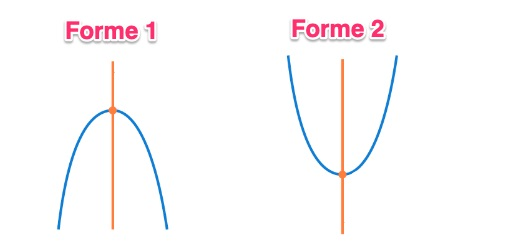
\includegraphics[width=0.6\linewidth]{/img/dst_01_forme.jpg}
  \caption{\label{} Formes de paraboles}
\end{figure}

\question[0.5] Donner la solution de l'équation dans $\mathbb{R}$ : $2x - 5 = -4x + 13$
\question[1] Factoriser l'expression $(5x - 2)(x+4) + 6(5x -2)$
\question[1] Dessiner le tableau de variation de la fonction $f$ définie sur l'intervalle $[-4 ; 4]$, et représentée dans le graphique ci-dessous : 

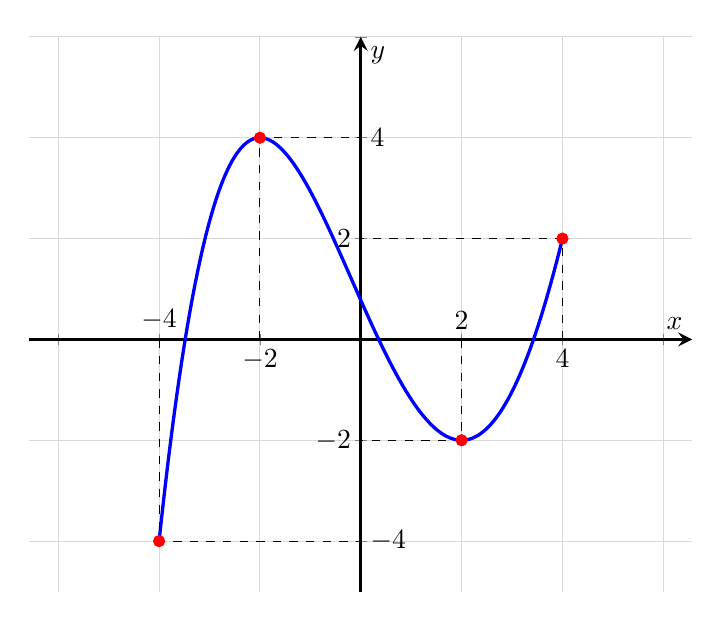
\begin{tikzpicture}[ 
  declare function={ 
  f(\x)=-(1/72)*\x^4+3/16*(\x^3)+(1/9)*\x^2-9/4*\x+7/9; 
  } 
  ]
  \begin{axis}[axis equal, 
  width=10 cm, 
  grid=major, 
  axis x line=middle, axis y line=middle, 
  axis line style = very thick, 
  grid style={gray!30}, 
  ymin=-5, ymax=6, yticklabels={}, ylabel=$y$, 
  xmin=-4, xmax=4, xticklabels={}, xlabel=$x$, 
  samples=500, 
  ] 
  \addplot[blue, very thick,domain=-4:4, smooth]{f(x)}; 
  \addplot [color=red, mark=*,only marks,samples at={-4,-2,2,4}] {f(x)}; 
  \pgfplotsinvokeforeach{-4,-2,2,4}{\draw[dashed] ({#1},0) |- (0,{f(#1)}); }
  \foreach \X/\Y in {-4/right,-2/left,2/left,4/right} 
  {\edef\temp{\noexpand\node[\Y] at (0,\X) {$\X$};} 
  \temp}
  \foreach \X/\Y in {-4/above,-2/below,2/above,4/below} 
  {\edef\temp{\noexpand\node[\Y] at (\X,0) {$\X$};} 
      \temp} 
  \end{axis}
  \end{tikzpicture} \par

  \begin{tikzpicture}
    \tkzTabInit{$x$ / 1 , $f(x)$ / 2}{\dots, \dots, \dots, \dots}
    %\tkzTabVar{-/ \textcolor{green}{$-4$}, +/\textcolor{red}{$4$}, -/$-2$, +/$2$}
 \end{tikzpicture}

 \question[1] Dresser le tableau de signe de la fonction $k$ définie sur $\mathbb{R}$ par : $k(x) = 3(x-4)(x+1)$. \textbf{Attention : le tableau ci-dessous est indicatif, il se peut qu'il manque quelques éléments dessus. A vous de les trouver} \par
\vspace{1em}
 \begin{tikzpicture}
  \tkzTabInit{$x$ / 1 , $k(x)$ / 1}{\dots, \dots, \dots, \dots}
  \tkzTabLine{, \dots, t, \dots, t,\dots }
\end{tikzpicture}

\end{questions}

\section{Exercice 2 - Etude d'une fonction}

\begin{questions}

\question[2] Montrer que la fonction $f(x) = -2x^2 - 4x + 16$ peut s'écrire sous la forme 
\[
-2(x-2)(x+4)
\]

\question[1] En déduire les solutions de l'équation $f(x)=0$

\question[1] Quelle est l'image de $x=3$ par la fonction f ?
\question[1] Le point $A$ de coordonées $(-1 ; 18)$ appartient-il à la courbe représentative de $f$ ? Qu'en est-il du point $B$ de coordonées $(0 ; 14)$ ? Justifier
\question[2] Construire le tableau de signe de la fonction $f$ sur le domaine de définition $\mathcal{D} = ] - \infty ; + \infty [$
\question[1] En déduire les solutions de l'inéquation 
\[
f(x) \geq 0
\]
On prendra le soin de bien écrire les intervalles

\question[1] L'extremum de la fonction (c'est-à-dire le maximum ou le minimum - on déterminera ce qu'il en est dans la question suivante) $f$ est atteint en $x = -1$. Dessiner le tableau de variation de la fonction $f$. \textbf{[Bonus à 0.5 point]} \textit{(sauter cette question bonus si vous n'avez pas la réponse, n'y passez pas trop de temps)} : à partir de la forme développée de la fonction $f$, comment aurions-nous pu trouver que l'extremum était atteint en $x=-1$ ?

\question[1] (Cette question se décompose en 3 sous questions) 
  \begin{itemize}
    \item Quel est le nombre de solutions de l'équation $f(x) = 20$ ?
    \item Quel est le nombre de solutions de l'équation $f(x) = 18$ ?
    \item Quel est le nombre de solutions de l'équation $f(x) = 2$ ?
  \end{itemize}


\end{questions}


\section*{Exercice 3 - Polynôme de degré 3 - Interpolation}


Soit la fonction polynôme de degré 3 $h$ définie dans $\mathbb{R}$ par :
\[
h(x) = x^3 - 2x^2 -x + d
\]
où $d$ est un paramètre à déterminer. On appelle $\mathcal{H}$ la courbe représentative de la fonction $h$. On souhaite imposer la contrainte suivante : La courbe \(\mathcal{H}\) doit passer par le point $B$ de coordonées $(1, 0)$.

\begin{questions}

\question[1] Montrer que $d = 2$
\question[1] Montrer que h peut s'écrire sous la forme factorisée : 
\[
  h(x) = (x-1)(x-2)(x+1)
\]

\question[1] Quel est le tableau de signe de la fonction $h$ sur le domaine de définition $\mathcal{D} = ] - \infty ; + \infty [$?
\question[1] Dans le graphique en dernière page, la courbe verte représente la fonction $f$ d'équation $f(x) = x^3 - 2x^2$. Montrer que la courbe rouge qui représente la fonction $g$ a pour équation 
\[
g(x) = x - 2
\]
\question[1] A partir de la question 3, résoudre l'inéquation suivante dans $\mathcal{D}$
\[
x^3 - 2x^2 \leq x - 2
\]
Quelle est l'interprétation graphique des résultats ?

\end{questions}

\begin{figure}[H]
  \centering
  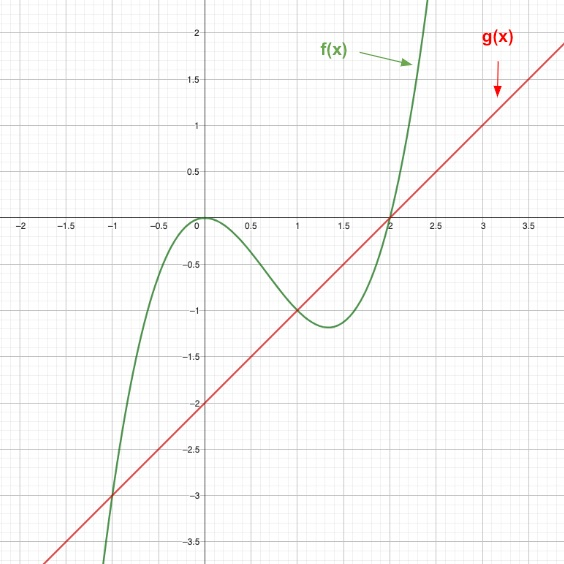
\includegraphics[width=\linewidth]{/img/dst_01_fonctions.jpg}
  \caption{\label{} Graphique de l'exercice 3}
\end{figure}


\end{document}


